\documentclass{beamer}
\usetheme{Frankfurt}
\usepackage{amsmath}
\usepackage{graphicx}
\usepackage{algorithm}
\usepackage{algpseudocode}
\usepackage{simplewick}
\usepackage{biblatex}
\usepackage{bbding}
\usepackage{xcolor}
\usepackage{caption}
\usepackage{subcaption}
\usepackage{tikz}
\usetikzlibrary{shapes.geometric, arrows}
\tikzstyle{startstop} = [rectangle, rounded corners, minimum width=2cm, minimum height=.7cm,text centered, draw=black, fill=red!30]
\tikzstyle{io} = [trapezium, trapezium left angle=70, trapezium right angle=110, minimum width=2cm, minimum height=.7cm, text centered, draw=black, fill=blue!30]
\tikzstyle{process} = [rectangle, minimum width=3.2cm, minimum height=1cm, text centered, text width=3cm, draw=black, fill=orange!30]
\tikzstyle{decision} = [diamond, minimum width=2cm, minimum height=.7cm, text centered, draw=black, fill=green!30]
\tikzstyle{arrow} = [thick,->,>=stealth]
\renewcommand*{\bibfont}{\tiny}
\setbeamertemplate{footline}[frame number]
\beamertemplatenavigationsymbolsempty
\graphicspath{{/home/raulquinteromonsebaiz/Documents/wickpresentation} }

\usepackage[utf8]{inputenc}

\author{Raul QUINTERO}
\title{Wick theorem for coupled cluster and for equation of motion coupled cluster}
\institute{LCPQ}

% logo of my university
\titlegraphic{
\includegraphics[width=4cm]{ERC}\hspace*{4cm}~%
   
\includegraphics[width=4cm]{Fermi}
}

\begin{document}

\begin{frame}
\titlepage
\end{frame}




\begin{frame}
\frametitle{Schrödinger equation}

\begin{itemize}
\item We work with the stationary Schrödinger equation in the Born-Openheimer approximation
\[ 
\hat{\mathcal{H}} | \Psi\rangle=E| \Psi\rangle
\]

\item $ | \Psi\rangle$ is the N-electron  wave function

\item $ \hat{\mathcal{H}}$ is the Exact Hamiltonian that contains the the N-electron kinetic energy and the electron electron interaction term

\[
\hat{\mathcal{H}}=  \hat{\mathcal{T}}+\hat{\mathcal{W}}
\]

\end{itemize}

\end{frame}










\begin{frame}
\frametitle{Second Quantization:Exact wavefunction}
\[
 | \Psi_{cc} \rangle = e^{\hat{T}} | \Psi_{0}  \rangle
 \]
Doing the cluster expansion of the exponential operator we obtain
 \[
 | \Psi_{cc} \rangle = \left(1+\frac{1}{2!} \hat{T}^{2}+\frac{1}{3!} \hat{T}^{3} + ...   \right)  | \Psi_{0} \rangle 
 \]

 Where the cluster operator is $ \hat{T}$
  
\[
 \hat{T}= \hat{T}_{1}+ \hat{T}_{2}+\hat{T}_{3}+...
\]
 
\[
 \hat{T}_{1} = \sum_{i,a}t^{a}_{i} \{ \textcolor{black}{\hat{a}^{\dagger}}\textcolor{black}{\hat{i}} \}
  \qquad 
   \hat{T}_{2}=\frac{1}{4} \sum_{i,j,a,b}t^{ab}_{ij}\{ \textcolor{black}{\hat{a}^{\dagger}}\textcolor{black}{\hat{i}}\textcolor{black}{\hat{b}^{\dagger}}\textcolor{black}{\hat{j}} \} 
\]

 
the indexes $\{i,j,k, \ldots  \}$ take in to account the occupied orbitals and  $\{a,b,c, \ldots  \}$ virtual orbitals. 
\end{frame}









\begin{frame}
\frametitle{Second Quantization: Excitation operators}

\begin{itemize}
\item  We can define the Hamiltonian  in normal order with respect the HF reference determinant 
 \[
\hat{\mathcal{H}}=\sum_{pq}h_{pq}\textcolor{orange}{ \hat{p}^{\dagger}\hat{q}}+\frac{1}{4}\sum_{pqrs} \langle pq || rs \rangle \textcolor{orange}{ \hat{p}^{\dagger}\hat{q}^{\dagger}\hat{s}\hat{r}}
\]
using the Wick Theorem:
 \[
\hat{\mathcal{H}}=\sum_{pq}f_{pq} \{\textcolor{orange}{ \hat{p}^{\dagger}\hat{q}} \}+\frac{1}{4} \sum_{pqrs} \langle pq || rs \rangle  \{ \textcolor{orange}{ \hat{p}^{\dagger}\hat{q}^{\dagger}\hat{s}\hat{r}} \}+ \langle 0 |\hat{\mathcal{H}}|0 \rangle 
\]
 \[
\hat{\mathcal{H}}=\hat{\mathcal{H}}_{N}+ \langle 0 |\hat{\mathcal{H}}|0 \rangle  \implies  \hat{\mathcal{H}}_{N}= \hat{\mathcal{H}} - \langle 0 |\hat{\mathcal{H}}|0 \rangle 
\]

\item The advantage of using the Hamiltonian in normal order is that \textcolor{blue}{ we can compute a product of strings without moving the indices that belong to the reference}
\end{itemize}

\end{frame}



























































\begin{frame}
\frametitle{Foundations in Coupled Cluster}
To solve  the Schr\"{o}dinger equation we  use the Normal Order Hamiltonian in the following way

\begin{equation}
   \hat{\mathcal{H}}_{N} e^{\hat{T}} | \Psi_{0} \rangle = \Delta E e^{\hat{T}} | \Psi_{0} \rangle 
\end{equation}

To calculate the energy we need the amplitudes, so we can project the Schr\"{o}dinger equation in the reference and excited determinants 


\[
 \langle \Psi_{0} | e^{-\hat{T}}  \hat{\mathcal{H}}_{N} e^{\hat{T}} | \Psi_{0} \rangle = \Delta E 
\]


\vspace{-10pt}
\[
\langle \Psi^{\textcolor{red}{ab}\ldots}_{\textcolor{blue}{ij}\ldots} |  \left( \hat{\mathcal{H}}_{N} e^{\hat{T}} \right)_{C}| \Psi_{0} \rangle = 0
\]


\end{frame}



\begin{frame}
\frametitle{Similarity Transformed Hamiltonian  in Coupled Cluster}

\begin{footnotesize}
\begin{itemize}
\item A more explicit form of the Similarity Transform Hamiltonian we can use the Backer-Campbell-Hausdorff Expansion.

\[
\left( \hat{\mathcal{H}}_{N} e^{\hat{T}} \right)_{C}= \hat{\mathcal{H}}_{N} + \left[ \hat{\mathcal{H}}_{N},\hat{T} \right]+\frac{1}{2}\left[ \left[ \hat{\mathcal{H}}_{N},\hat{T} \right],\hat{T} \right] +\frac{1}{3!}\left[\left[ \left[ \hat{\mathcal{H}}_{N},\hat{T} \right],\hat{T} \right] ,\hat{T} \right] 	+ 
\]
\begin{equation}
\frac{1}{4!}\left[\left[\left[ \left[ \hat{\mathcal{H}}_{N},\hat{T} \right],\hat{T} \right] ,\hat{T} \right],\hat{T} \right]
\end{equation}

\begin{equation}
\left( \hat{\mathcal{H}}_{N} e^{\hat{T}} \right)_{C}=e^{-\hat{T}}  \hat{\mathcal{H}}_{N} e^{\hat{T}}=   \hat{\mathcal{H}} +   \contraction{} { \hat{\mathcal{H}}}{}{ {\hat{T}}} 
  \hat{\mathcal{H}} \hat{T} + 
 \frac{1}{2}\contraction{}{ \bar{11}}{}{\bar{1}} 
    \contraction{} { \bar{11}}{1}{ {\hat{11}}} 
 \hat{\mathcal{H}} \hat{T} \hat{T}  +
\frac{1}{3!}  \contraction{}{ \bar{11}}{}{\bar{1}} 
    \contraction{} { \bar{11}}{1}{ {\hat{11}}} 
 \contraction{} { \bar{11}}{1}{ {\hat{11}}}
 \contraction{} { \bar{11}}{1}{ {\hat{111111}}}
\hat{\mathcal{H}} \hat{T} \hat{T} \hat{T}  +
\frac{1}{4!}  \contraction{}{ \bar{11}}{}{\bar{1}} 
    \contraction{} { \bar{11}}{1}{ {\hat{11}}} 
 \contraction{} { \bar{11}}{1}{ {\hat{11}}}
 \contraction{} { \bar{11}}{1}{ {\hat{111111}}}
 \contraction{} { \bar{11}}{1}{ {\hat{111111111}}}
\hat{\mathcal{H}} \hat{T} \hat{T} \hat{T}  \hat{T} 
\end{equation}
\item \textcolor{red}{The terms that are not connected contain partial contractions}
Example:
\[
\contraction{}{ \bar{11}}{}{\bar{1}} 
    \contraction{} { \bar{11}}{1}{ {\hat{11}}} 
 \contraction{} { \bar{11}}{1}{ {\hat{11}}}
\hat{\mathcal{H}} \hat{T} \hat{T} \textcolor{red}{ \hat{T}} 
\]
\end{itemize}

\end{footnotesize}


\end{frame}













\begin{frame}
\frametitle{Similarity Transformed Hamiltonian  in Coupled Cluster}



Using the connected similarity Hamiltonian in the projected equations


\[
\langle \Psi^{\textcolor{red}{ab}\ldots}_{\textcolor{blue}{ij}\ldots} |  \left(
 \hat{\mathcal{H}} +   \contraction{} { \hat{\mathcal{H}}}{}{ {\hat{T}}} 
  \hat{\mathcal{H}} \hat{T} + 
 \frac{1}{2}\contraction{}{ \bar{11}}{}{\bar{1}} 
    \contraction{} { \bar{11}}{1}{ {\hat{11}}} 
 \hat{\mathcal{H}} \hat{T} \hat{T}  +
\frac{1}{3!}  \contraction{}{ \bar{11}}{}{\bar{1}} 
    \contraction{} { \bar{11}}{1}{ {\hat{11}}} 
 \contraction{} { \bar{11}}{1}{ {\hat{11}}}
 \contraction{} { \bar{11}}{1}{ {\hat{111111}}}
\hat{\mathcal{H}} \hat{T} \hat{T} \hat{T}  +
\frac{1}{4!}  \contraction{}{ \bar{11}}{}{\bar{1}} 
    \contraction{} { \bar{11}}{1}{ {\hat{11}}} 
 \contraction{} { \bar{11}}{1}{ {\hat{11}}}
 \contraction{} { \bar{11}}{1}{ {\hat{111111}}}
 \contraction{} { \bar{11}}{1}{ {\hat{111111111}}}
\hat{\mathcal{H}} \hat{T} \hat{T} \hat{T}  \hat{T} 
 \right)_{C}| \Psi_{0} \rangle = 0
\]

Selecting one of the products of the expansion


\[
\langle \Psi^{\textcolor{red}{ab}\ldots}_{\textcolor{blue}{ij}\ldots} |  \left(
\contraction{}{ \bar{11}}{}{\bar{1}} 
    \contraction{} { \bar{11}}{1}{ {\hat{11}}} 
 \hat{\mathcal{H}} \hat{T} \hat{T} 
\right)_{C}| \Psi_{0} \rangle
\]







\end{frame}




\begin{frame}
An explicit example of the contraction is the following

\[
\langle \Psi^{\textcolor{red}{ab}\ldots}_{\textcolor{blue}{ij}\ldots} |  \left(
\contraction{}{ \bar{11}}{}{\bar{1}} 
    \contraction{} { \bar{11}}{1}{ {\hat{11}}} 
 \hat{\mathcal{H}} \hat{T} \hat{T} 
\right)_{C}| \Psi_{0} \rangle
\]

Selecting the simplest product of $\hat{T}\hat{T}$ 

\begin{footnotesize}
\[
 \sum_{kl\ldots,cd \ldots}\sum_{pqrs} \langle pq||rs \rangle \langle \Psi_{0} |\{ \textcolor{blue}{\hat{i}^{\dagger}} \textcolor{blue}{\hat{j}^{\dagger}} \ldots \textcolor{red}{\hat{a}} \textcolor{red}{\hat{b}} \ldots \} \{\textcolor{orange}{\hat{p}^{\dagger}\hat{q}^{\dagger}\hat{s}\hat{r}} \}
 \]
 \[
 \{\hat{c}^{\dagger}\hat{d}^{\dagger} \ldots \hat{k}\hat{l} \ldots \} \{ \hat{e}^{\dagger}\hat{f}^{\dagger} \ldots \hat{m}\hat{n}\ldots  \}| \Psi_{0} \rangle t_{kl \ldots}^{cd \ldots}t_{mn \ldots}^{ef \ldots}
\]
\end{footnotesize}

Expressing in a more simple notation
\[
\{
\textcolor{blue}{B^{\dagger}}\textcolor{red}{A}
\}
\{
\textcolor{orange}{H^{\dagger}}\textcolor{orange}{H}
\}
\{
T1^{\dagger}
T1
\}
\{
T2^{\dagger}
T2
\}
\]

\end{frame}



\begin{frame}
\frametitle{Wick theorem for coupled cluster}

\begin{footnotesize}
\begin{algorithmic}
\Require
\[
\{
\textcolor{blue}{B^{\dagger}}\textcolor{red}{A}
\}
\{
\textcolor{orange}{H^{\dagger}}\textcolor{orange}{H}
\}
\{
T1^{\dagger}
T1
\}
\{
T2^{\dagger}
T2
\}
\]
\State 1.
Obtain all the contractions between the different operators and separate them according the first operator

 
\State
2. Obtain all the possibilities between different subsets without repeating  operators. The simplest examples is $N[\textcolor{blue}{B^{\dagger}}]=1$,$N[\textcolor{red}{A}]=1$, $N[T1]=N[T2]=N[T1^{\dagger}]=N[T2^{\dagger}]
=1$
\[
\{
\textcolor{blue}{B^{\dagger}}
\textcolor{orange}{H},
\textcolor{red}{A}
T2^{\dagger},
\textcolor{orange}{H}
T1^{\dagger},
\textcolor{orange}{H^{\dagger}}
T2,
\textcolor{orange}{H^{\dagger}}
T1
\},
\{
\textcolor{blue}{B^{\dagger}}
T1,
\textcolor{red}{A}
\textcolor{orange}{H^{\dagger}},
\textcolor{orange}{H^{\dagger}}
T2,
\textcolor{orange}{H}
T2^{\dagger},
\textcolor{orange}{H}
T1^{\dagger}
\},\ldots
\]
\State
3. Obtain the sign
\[
sgn= \prod_{i=\{
\textcolor{blue}{B^{\dagger}},\textcolor{red}{A},
\textcolor{orange}{H^{\dagger}},\textcolor{orange}{H},
T1^{\dagger},
T1,
T2^{\dagger},
T2,
\}}(-1)^{P_{in}[i]-P_{fin}[i]}
\]
where $P_{in}[i]-P_{fin}[i]$ is the initial positions minus the final position
\end{algorithmic}
\end{footnotesize}
\end{frame}



\begin{frame}
\frametitle{EE-EOMCCSD}

\begin{footnotesize}


We can diagonalize the similarity transformed Hamiltonian in a CISD basis to obtain the EE-EOMCCSD
\[
\begin{pmatrix}
 \langle \Psi^{\textcolor{red}{a}}_{\textcolor{blue}{i}} | \bar{\mathcal{H}} |\Psi^{\textcolor{green}{c}}_{\textcolor{purple}{k}}  \rangle  &   
  \langle \Psi^{\textcolor{red}{a}}_{\textcolor{blue}{i}} | \bar{\mathcal{H}} |\Psi^{\textcolor{green}{cd}}_{\textcolor{purple}{kl}}  \rangle  
  \\ 
  \langle \Psi^{\textcolor{red}{ab}}_{\textcolor{blue}{ij}} | \bar{\mathcal{H}} |\Psi^{\textcolor{green}{c}}_{\textcolor{purple}{k}}  \rangle    & 
 \langle \Psi^{\textcolor{red}{ab}}_{\textcolor{blue}{ij}} | \bar{\mathcal{H}} |\Psi^{\textcolor{green}{cd}}_{\textcolor{purple}{kl}}  \rangle 
\end{pmatrix}
\begin{pmatrix}
s^{\textcolor{green}{c}}_{\textcolor{purple}{k}}\\
s^{\textcolor{green}{cd}}_{\textcolor{purple}{kl}}
\end{pmatrix}=\omega_{\lambda}
\begin{pmatrix}
s^{\textcolor{green}{c}}_{\textcolor{purple}{k}}\\
s^{\textcolor{green}{cd}}_{\textcolor{purple}{kl}}
\end{pmatrix}
\]

We are interested in computing the elements like this:


\[
 \langle \Psi^{\textcolor{red}{ab}}_{\textcolor{blue}{ij}} | \bar{\mathcal{H}} |\Psi^{\textcolor{green}{cd}}_{\textcolor{purple}{kl}}  \rangle 
\]

Expanding the similarity transformed Hamiltonian we obtain


\[
\langle \Psi^{\textcolor{red}{ab}}_{\textcolor{blue}{ij}} |  \left(
 \hat{\mathcal{H}} +   \contraction{} { \hat{\mathcal{H}}}{}{ {\hat{T}}} 
  \hat{\mathcal{H}} \hat{T} + 
 \frac{1}{2}\contraction{}{ \bar{11}}{}{\bar{1}} 
    \contraction{} { \bar{11}}{1}{ {\hat{11}}} 
 \hat{\mathcal{H}} \hat{T} \hat{T}  +
\frac{1}{3!}  \contraction{}{ \bar{11}}{}{\bar{1}} 
    \contraction{} { \bar{11}}{1}{ {\hat{11}}} 
 \contraction{} { \bar{11}}{1}{ {\hat{11}}}
 \contraction{} { \bar{11}}{1}{ {\hat{111111}}}
\hat{\mathcal{H}} \hat{T} \hat{T} \hat{T}  +
\frac{1}{4!}  \contraction{}{ \bar{11}}{}{\bar{1}} 
    \contraction{} { \bar{11}}{1}{ {\hat{11}}} 
 \contraction{} { \bar{11}}{1}{ {\hat{11}}}
 \contraction{} { \bar{11}}{1}{ {\hat{111111}}}
 \contraction{} { \bar{11}}{1}{ {\hat{111111111}}}
\hat{\mathcal{H}} \hat{T} \hat{T} \hat{T}  \hat{T} 
 \right)_{C}|\Psi^{\textcolor{green}{cd}}_{\textcolor{purple}{kl}}  \rangle = 0
\]

Using the previous  product of  $\hat{T}\hat{T}$ 

\[
\langle \Psi^{\textcolor{red}{ab}}_{\textcolor{blue}{ij}} |  \left(
 \frac{1}{2}\contraction{}{ \bar{11}}{}{\bar{1}} 
    \contraction{} { \bar{11}}{1}{ {\hat{11}}} 
 \hat{\mathcal{H}} \hat{T} \hat{T} 
 \right)_{C}|\Psi^{\textcolor{green}{cd}}_{\textcolor{purple}{kl}}  \rangle = 0
\]

Using the simplified notation

\[
\{
\textcolor{blue}{B^{\dagger}}
\textcolor{red}{A}
\}
\{
\textcolor{orange}{H^{\dagger}}\textcolor{orange}{H}
\}
\{
T1^{\dagger}
T1
\}
\{
T2^{\dagger}
T2
\}
\{
\textcolor{green}{C^{\dagger}}
\textcolor{purple}{D}
\}
\]

\end{footnotesize}
\end{frame}






\begin{frame}
\frametitle{Wick theorem for EE-EOMCCSD}

\begin{footnotesize}


Using the simplified notation

\[
\{
\textcolor{blue}{B^{\dagger}}
\textcolor{red}{A}
\}
\{
\textcolor{orange}{H^{\dagger}}\textcolor{orange}{H}
\}
\{
T1^{\dagger}
T1
\}
\{
T2^{\dagger}
T2
\}
\{
\textcolor{green}{C^{\dagger}}
\textcolor{purple}{D}
\}
\]

Now we have two different contractions:
\begin{itemize}
\item The external contractions: are made with respect the bra and the ket, and are all the possible CONECTED contractions considering $N[\textcolor{blue}{B^{\dagger}}`]=N[\textcolor{red}{A}]=N[\textcolor{green}{C^{\dagger}}]=N[\textcolor{purple}{D}]=2$


\[
\left[
\left(
\textcolor{blue}{B^{\dagger}}
\textcolor{purple}{D}
\right),
\left(
\textcolor{red}{A}
\textcolor{green}{C^{\dagger}}
\right)
\right],
\]
\[
\left[
\left(
\textcolor{blue}{B^{\dagger}}
\textcolor{purple}{D},
\textcolor{blue}{B^{\dagger}}
\textcolor{purple}{D}
\right),
\left(
\textcolor{red}{A}
\textcolor{green}{C^{\dagger}},
\textcolor{red}{A}
\textcolor{green}{C^{\dagger}}
\right)
,
\left(
\textcolor{red}{A}
\textcolor{green}{C^{\dagger}},
\textcolor{blue}{B^{\dagger}}
\textcolor{purple}{D}
\right), \ldots
\right],
\]
\[
\left[
\left(
\textcolor{blue}{B^{\dagger}}
\textcolor{purple}{D},
\textcolor{blue}{B^{\dagger}}
\textcolor{purple}{D},\textcolor{red}{A}
\textcolor{green}{C^{\dagger}}
\right),
\left(
\textcolor{red}{A}
\textcolor{green}{C^{\dagger}},
\textcolor{red}{A}
\textcolor{green}{C^{\dagger}},
\textcolor{blue}{B^{\dagger}}
\textcolor{purple}{D}
\right)
,\ldots
\right]
\]

\item The internal contraction are made for each external. They are made by the rest of strings for a given external. The Wick theorem for coupled cluster is used for each internal  

\end{itemize}
\end{footnotesize}
\end{frame}







\begin{frame}
\frametitle{Categorize the integrals : Example}
\begin{footnotesize}
\begin{algorithmic}

\State 7. Categorize the integrals and amplitudes to obtain all the diagrams (programmable expressions)


\[
\langle \Psi^{\textcolor{red}{ab}}_{\textcolor{blue}{ij}} |  \hat{\mathcal{W}}_{N} \hat{T}_{1}^{2}   | \Psi_{0} \rangle 
\]
\[
=\frac{1}{8} \sum_{kl,cd}\sum_{pqrs} \langle pq||rs \rangle \langle \Psi_{0} |\{ \textcolor{blue}{\hat{i}^{\dagger}}\textcolor{red}{\hat{a}}\textcolor{blue}{\hat{j}^{\dagger}}\textcolor{red}{\hat{b}} \} \{\textcolor{orange}{\hat{p}^{\dagger}\hat{q}^{\dagger}\hat{s}\hat{r}} \}\{\hat{c}^{\dagger}\hat{k} \} \{ \hat{d}^{\dagger}\hat{l} \}| \Psi_{0} \rangle t_{k}^{c}t_{l}^{d}
\]







\State Mathematica output after Wick theorem

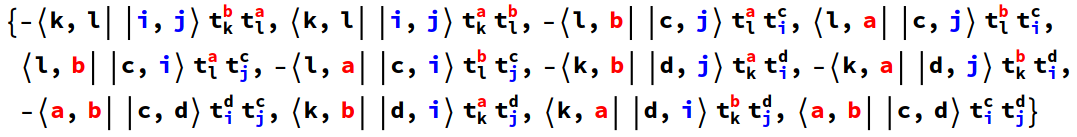
\includegraphics[scale=.2]{sort1}

\State Sorting the classes of terms with respect color an position


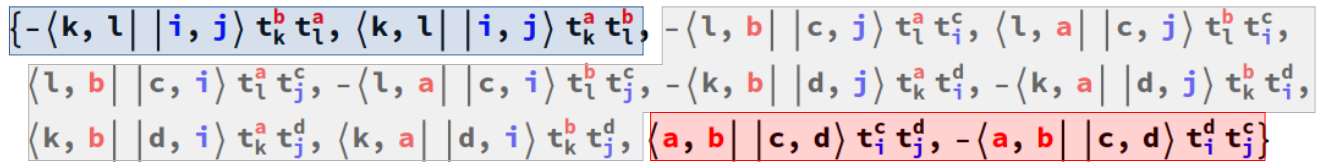
\includegraphics[scale=.17]{sort2}

\State  Play with the dummy indexes


\[
\langle \Psi^{\textcolor{red}{ab}}_{\textcolor{blue}{ij}} |  \hat{\mathcal{W}}_{N} \hat{T}_{1}^{2}   | \Psi_{0} \rangle = \sum_{kl} \langle kl||\textcolor{blue}{ij} \rangle  t_{k}^{\textcolor{red}{a}}t_{l}^{\textcolor{red}{b}} +P(i,j,a,b)\sum_{k,c} \langle k \textcolor{red}{a}||c\textcolor{blue}{i} \rangle  
t_{k}^{ \textcolor{red}{b} }t_{ \textcolor{blue}{j}}^{c}+\sum_{cd} \langle  \textcolor{red}{ab}||cd \rangle  
t_{\textcolor{blue}{i}}^{ c }t_{ \textcolor{blue}{j}}^{d}
\]







\end{algorithmic}


\end{footnotesize}

\end{frame}

















\begin{frame}
\frametitle{Categorize the integrals : Example}
\begin{footnotesize}
\begin{algorithmic}

\State 7. Categorize the integrals and amplitudes to obtain all the diagrams (programmable expressions)








\[
\langle \Psi^{\textcolor{red}{ab}}_{\textcolor{blue}{ij}} |  \hat{\mathcal{W}}_{N} \hat{T}_{1}^{2}   | \Psi_{0} \rangle = \sum_{kl} \langle kl||\textcolor{blue}{ij} \rangle  t_{k}^{\textcolor{red}{a}}t_{l}^{\textcolor{red}{b}} +P(i,j,a,b)\sum_{k,c} \langle k \textcolor{red}{a}||c\textcolor{blue}{i} \rangle  
t_{k}^{ \textcolor{red}{b} }t_{ \textcolor{blue}{j}}^{c}+\sum_{cd} \langle  \textcolor{red}{ab}||cd \rangle  
t_{\textcolor{blue}{i}}^{ c }t_{ \textcolor{blue}{j}}^{d}
\]


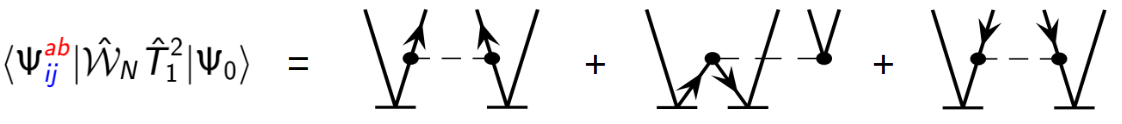
\includegraphics[scale=.22]{sumdiag}


After classifying by the indexes that belong to the bra, playing with the dummy indexes and factorizing we can obtain the Goldstone diagrams, that represent the interaction between the Hamiltonian and excitation operators.

\end{algorithmic}
\end{footnotesize}


\end{frame}


\begin{frame}
\frametitle{Conclusions}
\begin{itemize}
\item A symbolic algebra program to obtain Coupled Cluster is described 
\item A procedure to contract an arbitrary number of second-quantization expressions and simplify them to map analytical result in to diagrams
\end{itemize}

\end{frame}




\end{document}
